\documentclass[11pt,letterpaper]{refart}
\usepackage{graphicx}
\usepackage{amssymb}
\usepackage{epstopdf}
\usepackage{xcolor}
\usepackage{array}
\usepackage[bookmarks]{hyperref}
\usepackage{pdfpages}	

\newenvironment{fulltable}[1][tbp]
 {\begin{table}[#1]%
  \hspace*{-\leftmarginwidth}%
  \begin{minipage}{\fullwidth}}
 {\end{minipage}\end{table}}
 \def\nada{\hspace{0pt}}

\DeclareGraphicsRule{.tif}{png}{.png}{`convert #1 `dirname #1`/`basename #1 .tif`.png}
\def\ui#1{\textsf{#1}}
\title{User Manual---Bridge Design Contest Administrator \\[1ex]
\small Engineering Encounters, Inc.}
\author{Gene Ressler}
\date{\today}

\setlength{\belowcaptionskip}{11pt}

\begin{document}
\maketitle
\tableofcontents\newpage

\section{Overview and Changes}
This document explains how to use the Engineering Encounters Bridge Design 
Contest Administrator
Interface or CAI. It covers only the CAI itself, assuming the reader already knows
about contest operations, policies, and procedures. The CAI is a web browser-based 
``window" into the contest database. Its design allows a small administrative
team to conduct the contest even if the number of participants is very large. 

Here is a brief overview of CAI functions:
\begin{itemize}
\item Create and activate automatic schedules for annual cycles of qualifying and semi-final rounds.*
\item Review and accept top teams.
\item Post official standings.
\item Set up local contests and view their current standings.
\item Establish team groups, where only the top team appears in standings.*
\item Inspect and analyze designs and download them.
\item Designate teams for the semi-final round and post contestant instructions.*
\item Query the contest database in various ways.
\item Generate Certificates of Achievement for local contest and qualifying round accomplishments.*
\item Send bulk emails.*
\item Manually disable the contest, with an explanatory message banner displayed at
 the login page.*
\item Serve maps showing the distribution of US contest participants.
\end{itemize}

\subsection{Changes}
The features above marked with asterisks (*) are new. Indeed, there are many 
changes in the CAI with respect to the original 1999 design. Some are
obvious. Others are subtle but still important. A brief overview follows. Those who
have never used the original CAI may safely skip to the next section.

Automatic schedules are new. In the old CAI, the milestone dates and times of contest 
rounds could be established only at the server console. Now they can be 
set in the CAI. 

Team groups are a new feature to support the 
``one winner per school" rule. 

Manual disabling of logins is another new facility that
has moved from the console to the CAI web interface, available to any Administrator
at any location.

The new CAI has \emph{persistent configuration}. Various options and
search criteria are automatically remembered between uses. Where the
old administrator had only one ``account," the new one allows any number
of administrator login names so that a different persistent configuration
can be saved for each.

The new CAI does not require setting up new, different accounts for semi-final teams. 
Instead, semi-finalists are merely marked in the Team Review portion of the CAI. 

In the new system, any team can participate in up to four local contests at any time.
These can be either 
4-character (all-scenario) or 6-character (scenario-specific) contests without regard for the 
current contest round. The old system allowed only 4-character contests 
during the Qualifying Round. That restriction is gone. Another quirk of the 
old system was that 6-character codes could not change after registration. This quirk is 
also gone. Teams can add and delete local contests at any time. 

This added flexibility results from added internal complexity. The new system tracks the  
best  design for each scenario for each team rather than only a single best per team in 
the old one. Formerly, a bridge submission was accepted by the system only if 
it improved on a team's current best (lowest cost) bridge overall. The definition of 
\emph{improvement} has changed in the new system: a bridge is an improvement, and 
therefore accepted in the new system, if it has cost
lower than all previous submissions by the team \emph{for the same scenario}. This
more liberal policy will probably cause more bridges to be accepted per team. 

Bulk email is now performed by the contest server. This is necessary to gain the benefit of
a registered bulk mail service that has much less chance of being blocked by spam detectors.
A new ``rich text" editor in the CAI allows messages with standard text formatting.
The rich text editor also allows documents with images. At present, however, these will
not work for bulk email.

Downloadable Certificates of Achievement that acknowledge and celebrate the standing 
that each team earns in the contest are also new. 

Other changes are for usability. 
\begin{itemize}
\item Team names that contain contestant last names are highlighted.
\item Design review, analysis, and download have been integrated with the review screen. 
\item Differences between currently posted and new standings can be displayed with 
  strikeouts and color coding in a manner similar to Microsoft Word revision marks. 
\item The local contest manager now protects against inadvertently choosing a local 
  contest code that is already in use.
\end{itemize}

\subsection{We need you}
The CAI remains a work in progress. If you're an Administrator and see something
that the CAI could do to make your life easier, tell the CAI software team.

\section{Key concepts}
Several key concepts are important to avoid mistakes and use the Administrator
efficiently.

\subsection{Administrators}
An Administrator is a person entrusted with contest administration and decision authority. 
Each Administrator has a user id and password for validating his or her identity. The 
password is initialized with an easy-to-guess value when the system is 
created. Therefore, each Administrator must immediately log in to change his or her password 
to a personal, difficult-to-guess value. The main purpose of Administrator accounts is to
store persistent information about the Administrator's preferences. 

Additionally, the separate logins allow individual activity to be tracked in the server logs. 
With the old Administrator, determining who performed a given Administrator 
function---occasionally useful---was difficult.

There is nothing to prevent more than one Administrator from logging in 
and making changes during the same period. This has always been true. 
External communication among Administrators is needed to prevent
confusion when one Administrator's view changes due to work done by
another at a different location.

Where the old CAI expected the user to close his or her browser to log out, the
new one has a log out feature. Its use is highly recommended for the obvious
security reasons. Administrator sessions never expire, unlike team logins, which
expire after a few minutes.

\subsection{Team categories}
Teams competing in the contest fall into only three categories in the new CAI.
\begin{description}
\item[US/PR High School Students]  PR is for Puerto Rico. This includes all 
grade 9 to 12
kids who are either attending US schools (regardless of national origin) or are
US citizens (regardless of location or school choice including home-schooling).
\item[US/PR Middle School Students]  This is the same as the High School
category above, except for grade 6 to 8 kids.
\item[Open Competition]  All people who are not US/PR High School
or Middle School students.
\end{description}
US/PR Students, both Middle and High School, are eligible for recognition, 
advancing through successive
contest rounds, and receiving prizes. Open competitors are in it for fun only.

Long-time contest participants will remember that categories once included the
four ASCE zones. Also, the old CAI presented Semi-finalists as a category.
Neither is currently true.

\subsection{Team status}
The status of a contest Team consists of four values. 
Each has an associated color to denote
it in the CAI.
\begin{description}
\item[Unreviewed (gray)] The team has successfully registered and 
uploaded at least one design,
but no Administrator has yet reviewed or advanced it to one of the three reviewed
states that follow.
\item[Rejected (red)] The team has been disqualified by an Administrator. 
Logins are permitted, but the Team Home Page contains only a message 
and Log Out link. No further uploads are possible.
\item[Accepted (green)] The team has been reviewed and deemed suitable
to continue in the competition. It can appear in official standings if its best
design has a high standing.
\item[Semi-final (purple)] An Administrator has designated the team as
a semi-final competitor. The status of such a team is identical to an Accepted
team except that during the Semifinal period, its home page is augmented
with Semi-final instructions and a chance to select between a Semi-Final-specific
home page and the team's normal qualifying round page. In the old system, the
Team could do the same by using either its normal or semi-finals-specific
user id. Here, the normal user id is used for all.
\end{description}
Semi-final status should be thought of as ``Accepted with benefits."  A Semi-final
team can continue to participate in local contests. Its local and national standings 
are unaffected by its semi-finalist status.

\subsection{Local contests}
Local contests are just collections of teams that have entered the same
4-\ or 6-character local contest code in the registration pages. Every
team can enter up to four local contests of either type or delete them 
at any time. The  system generates standings of all contestants for 
all local contests. These are updated every half-hour or so. Rejected teams 
do not appear.

Local contests have been run by teachers, home-school parent groups, 
principals, superintendents, college professors, states, and foreign countries.
The person who wishes to run the local contest emails an Administrator to 
obtain a code. He or she is responsible to 
communicate this code to the local contest competitors, who enter it in their
team registration information pages. Soon after successfully
submitting a design (of the correct design scenario for a 6-character contest), 
the team will appear in the local contest standings.

\subsection{Team groups}
In the new CAI, teams can be placed in named groups of arbitrary size. When
official standings are generated, only one team per group will appear---the
one with the highest standing among group members.

\subsection{Certificates}
\label{sec:certificates}
The CAI is capable of producing Certificates of Achievement for the
qualifying round (including a ribbon for semifinalists) and for each local contest.
Up to five certificates may be awared to each team---one for the qualifying round
and another for each of up to four local contests.

These appear as links on the team home page. Clicking the respective link
produces a PDF document in a fresh browser tab. Each certificate is suitable 
for high quality printing and display in an 8x10 inch frame. 

Certificates must be explicitly posted by an 
administrator for each local contest and for the qualifying round. They may also 
be revoked individually for each local contest and for the entire qualifying round. 

Most attributes of certificates are \emph{frozen} at the time the administrator creates
them. They do not change even if the team submits improved bridges or other
teams with higher standings are rejected. Frozen attributes include the standing 
and \emph{basis} (total number of competitors) for the local contest or qualifying round 
for the respective kind of certificates. For the qualifying round, the standing within 
the team's group (if any) is frozen and also the basis within the group.

Semifinalist ribbons not frozen. Updates to the semifinalist status of a team are 
reflected immediately in the qualifying round certificate.

Example certificates are presented in the Appendix, Section~\ref{sec:examplecertificates}.

\subsection{Data likenesses}
For several functions of the CAI, the user can enter a pattern known as a \emph{likeness}
to search for contest database records. A likeness is just text. When the likeness
\emph{matches} other text in the database, the data record (for a team, local contest,
group, etc.) containing the text is reported as a search result. Otherwise it is not. 
Likenesses are powerful because they assign special meaning to two characters:
percent (\texttt{\%}) and underscore (\texttt{\_}). These obey the rules shown in
Table~\ref{tbl:likeness}.\
\begin{table}
\centering
\caption{Characters in likenesses.}
\begin{tabular}{l>{\tt}cl}
\multicolumn{2}{l}{\bfseries Likeness character} & {\bfseries Matches\ldots} \\ \hline
Percent sign & (\texttt{\%}\nada) & any string of zero or more characters \\
Underscore  & (\texttt{\_}\nada)  & any single character \\
Any other character & $x$ & the same character $x$, ignoring case.
\end{tabular}
\label{tbl:likeness}
\end{table}

For example, \texttt{\%s\%hwa\_\%z} will match \texttt{Jerry Schwartz},
\texttt{Jansy Ohwaraz}, and many other data.

\section{Login and pattern of use}
The CAI login is available at the server address followed by \texttt{/admin}, currently
\begin{quote} 
\texttt{https:/judge.bridgecontest.org/admin}
\end{quote}
Enter your Administrator login and password and press the \ui{Log In} button.

Maximize your browser window, and note it is divided into two panes: the \emph{menu pane}
on the left and the \emph{display pane} on the right. The general pattern of CAI use is
to initiate a function by making a selection in the menu pane and then continue it
by reading and interacting with the display pane. When the menu item includes
a select box, merely changing the selection often invokes the selected function.
When this doesn't happen, or you wish to re-display the current selection, perhaps 
after selecting new options, press the  \ui{Go} button for the function.

\section{Options}
Nearly all CAI functions respond to the \ui{Options} selectors 
at the bottom of the menu. 

\subsection{Review and standings cutoff}
Various CAI functions present lists of contest team records as review boxes 
(see section~\ref{sec:reviewboxes}) and 
standings. The maximum number of records displayed is set in this option.
 
\subsection{Visible attributes}
\label{sec:reviewboxes}
Various CAI functions present \emph{review boxes}, one per team. The boxes
contain items of current team information called \emph{attributes}. 
The visibility of each attribute may be switched on and off the 
\ui{Visible attributes} selector. On Windows computers, 
hold the Control key down while selecting and de-selecting attributes. On Apple
computers, hold down the Command key. Otherwise
all attributes will be cleared except the last selection. Use the buttons next to 
the selector to select all, clear all, or reset the selector to its default values. The
available attribute names are self explanatory and correspond to information
provided by teams on their registration forms except for a few as described
in subsection \ref{sec:reviewboxes}.

For technical reasons, the review display will take considerably longer to compute
(perhaps a full second on the server side) if the \ui{Local contests}  and/or 
\ui{Best design} attributes are selected. Consider turning them off if the
information they provide is not needed.

\section{Maintenance functions}
The top row of menu links consist of functions to check, control and maintain the 
Administrator's use of the CAI.

\subsection{New password}
This menu item presents, in the display pane, an opportunity for the
the Administrator to change his or her CAI password.

\subsection{Server}
Selecting this menu item fills the display pane with information about the
current state of the contest servers (there are three of them).  

It also contains an experimental interface
for clearing the contest database.  For security reaons, this function is currently
not operational.

\subsection{Schedule}
This menu item causes the display pane to be filled with the \emph{schedule
manager}. The schedule manager controls what users see at the contest
login page and, after they are logged in, what they are able to do. 
It does so indirectly by allowing the administrator to specify a set of key 
date-times and other bits of information.
Overall, the manager has four related purposes.
\begin{itemize}
\item Starting and stopping the various rounds of the contest.
\item Posting or revoking Certificates of Achievement (see Section~\ref{sec:certificates}) 
  for the qualifying round.
\item Re-enabling logins after they are automatically turned off
as the qualifying round ends.
\item Temporarily disabling and re-enabling all logins with a banner 
message.
\end{itemize}
These are obviously powerful functions, so the schedule manager must
be used with great care.

A schedule consists of a list of sequential dates and other information
shown in Table~\ref{tbl:schedule}. This table depicts the flow of an
annual contest cycle. Banners on the login page indicate the current
status. For example, before qualifying round registration begins, the
banner gives the start date and encourages people to return. After
all rounds are complete, the banner exhorts teams to submit designs
for fun and return for next year's qualifying round.

Any number of schedules
may be prepared in advance using the \emph{schedule workspace}.
The workspace displays the values of one schedule---either a new
one that is being created or an existing one that is being updated.
Buttons at the bottom of the manager have functions described in the
following paragraphs.
\begin{fulltable}
\centering
\caption{Contest schedule information.}
\begin{tabular}{>{\sffamily}llp{9cm}}
\bfseries Schedule item & \bfseries Type & \bfseries Description \\ \hline 
Name & text & unique identifier for the schedule \\
Active & checkbox & checked for the currently active schedule \\
Start registration & date & users may register and log in but not submit designs \\
Start qualifying & date & users may register, log in, and submit designs \\
End qualifying & date & logins disabled until the \ui{Tally complete} box is checked \\
Tally complete & checkbox & when checked, logins are re-enabled after qualifying round end \\
Start semifinals logins & date & semifinalists can log in to either home page but not submit semifinal designs\\
Semifinals instructions & document & instructions page presented at each semifinal login\\
Start semifinals & date & semifinalists can log in only to semifinal page and submit designs \\
End semifinals & date & semifinalists can log in only to their regular home page \\
Suspend logins & checkbox & all logins are temporarily suspended \\
Banner message & text & displayed at login page while logins are suspended
\end{tabular}
\label{tbl:schedule}
\end{fulltable}

\subsubsection{Add schedule/Update schedule}
If the schedule workspace contains a new schedule, fill it in with schedule information
and press \ui{Add} to save the schedule in the contest database. If the
workspace contains an existing schedule, make changes and press \ui{Update}
to save them in the contest database.

If you add or update a schedule with \ui{Active} checked, the schedule becomes
immediately effective. The old active schedule is automatically deactivated.

\subsubsection{Get new or selected schedule}
To clear the workspace and fill it with a new schedule, ensure no 
review box is selected and press this button.

To retrieve an existing schedule into the workspace, select 
its review box and press this button. If more than one review box is
checked, only the first will be retrieved. 

\subsubsection{The active schedule and disabling logins}
At most one schedule can be active. If no schedule is active, then logins are disabled.
Activate any schedule by getting it into the workspace, checking the \ui{Active} box,
and pressing \ui{update}. The change is immediately effective.

To change the active schedule in any manner---for example, to suspend team logins
temporarily---retrieve it into the workspace, make the desired changes, and press
\ui{Update}. The change is immediately effective.

\subsubsection{Certificates for the Qualifying Round}
Buttons to post and revoke Certificates of Achievement (see 
Section~\ref{sec:certificates}) are presented in the schedule
workspace. Pressing them initiates background processing 
that eventually creates, re-creates, or deletes certificates for all qualifying
round teams that have submitted at least one design.

These buttons are positioned visually between the qualifying round end
date-time and the "Tally Complete" check box because posting
of qualifying round certificates is most logically done during the
period that the system is closed for qualifying round results 
tallying.

\subsubsection{Delete selected schedules}
To delete schedules, select all their review boxes and press this button
once. You'll be asked if you're sure you wish to proceed. Deletions cannot
be undone, so be sure. The active schedule cannot be deleted.

\subsection{Qualogin}
A contraction for ``Qualifying round login," select this option to obtain the
team login and registration page even if the contest is closed for logins 
according to the active schedule. In this pseudo-qualifying round, you can 
register teams and submit designs until the administrator session is 
terminated by logging out or closing the browser.

\subsection{Logout}
This menu item terminates the Administrator's session with the CAI.

\section{Team review}
This section describes the CAI's support for reviewing teams and advancing
them from the Unreviewed status to one of the three reviewed ones: rejected,
accepted, or semi-final. The status of a team may change more than once as
the contest proceeds including ``backward'' to the unreviewed status.

Review begins by selecting a category from the CAI menu using the box labeled
\ui{Review (Accept/Reject) top teams}. Press \ui{Go} if necessary to fill
the display pane with review boxes for the top $N$ teams, where $N$ is the number
in the \ui{Review cutoff} selector. 

\subsection{Index}
The index at the top of the display is a table of marks, one per review box. The 
mark is a numeric \emph{standing}, an \ui{x}, or an \ui{o}, depending on the status of
the team. The mark is also a link. Clicking it scrolls down to the respective team
review box. Each review box header contains a $[\hbox{\ui{top}}]$ link to scroll
back to the index. The mark is an \ui{x} if the team's status is unreviewed or
rejected. Otherwise the team has a status of accepted or semi-final. In these 
cases, the mark will be the numerical standing of the team nationally in its
category.

The sole exception occurs when the team is in the same group as a 
team with higher standing. In this case the mark is an \ui{o}.

\subsection{Processing}
Immediately below the index is a button marked \ui{Process}. After you've 
completed a review by changing status and group settings as described below
in section~\ref{sec:heading}, press this button to record them in the database. 

Any number of changes will be recorded by a single press of the button.
They take effect immediately. For example, teams that are rejected will no longer be 
able to submit designs, and their home pages will show a message explaining that 
they've been disqualified.

\subsection{Review box}
Each team is described by a review box. The box also includes controls to change
the team's status. Parts of the review box are explained in subsequent paragraphs.

\subsubsection{Standing bar}
The standing bar is the left border of the review box. Its color and mark match
its Index entry as describe above. 

\subsubsection{Heading}
\label{sec:heading}
The heading is the top border of the review box. It contains both information
and controls that record your review of the team. 

\paragraph{Name key}
This is the team name
with all but letters and digits removed and letters converted to lower case. The
system ensures that name keys (not just team names) are unique in any contest 
round. If the name key text is red, the Administrator
should inspect it carefully, because this means the CAI has detected that at
least one of the members' family names is embedded in the team name. Green
highlighting shows the characters that must be inserted in the family name to
obtain the team name. For example, if the team name is \ui{**SxMxIxTxH**}, and
one of the members is named Smith, then the name key will be portrayed as
\ui{\color{red}{sxmxixtxh}}, with the \ui{x}es highlighted in green.

\paragraph{Unofficial standing}
This shows the unofficial standing that will be reported to the team on its home
page. Unofficial standings assign a standing to a team regardless of its status 
unless it is rejected. They also ignore team groups. Official standings for 
the national contest show only teams
that are in the accepted or semi-final status, and they award a standing only to
the top team in each group. Due to the differences between the two ways 
standings are computed, official standings are often better (that is, the ranking 
number is smaller) than unofficial ones.

\paragraph{Group selector}
This control lists all team groups in the contest. (The current list
of groups is maintained by another CAI function.)
To add a team to a group, merely 
change its selector from \ui{No group selected} to one of the other choices. You 
can reverse this at any time by re-choosing \ui{No group selected}. In either case,
don't forget to press \ui{Process} to record your changes. Among all teams
in a group, only the one with the best design will appear in official standings.

\paragraph{Status selector}
The current status of the team may be changed by selecting the appropriate
radio button. Changes take effect immediately after the \ui{Process} button is
pressed. Email messages to teams are automatically generated under the 
following circumstances:
\begin{description}
\item[Disqualification] The team's status changes to rejected from some other status.
\item[Qualification] The team's status changes to either accepted or
semi-final from another status that's not either of these two.
\end{description}
These messages are personalized for the team, but their contents are currently
``hard wired" into the CAI. Editing them requires coordination with the CAI 
author.

\paragraph{Top link}
This is just a link that causes the display pane to scroll all the way to the top.
Normal uses are to reach the index in order to skip to a different team's record
and to display the \ui{Process} button so that status or group selector changes
can be recorded in the database.

\subsubsection{Attributes}
The rest of the review box lists attributes of the team in tabular form. The visibility of attributes
may be changed using the \ui{Options} selector in the menu pane. These attributes
are taken directly from information provided by the team during registration with a 
few additions as follows:
\begin{description}
\item[Status] The current status of the team, which is also visible in the 
color of the \emph{standing bar}.
\item[Registration] The date and time team registration was completed.
\item[Best score] The cost of the least expensive bridge submitted by the team so far.
\item[Best design] A small sketch of the best bridge submitted by the team with links
to a corresponding \emph{structural analysis table} and \emph{bridge file download}.
The table format is identical to the West Point Bridge Designer's. Bridge file downloads 
may be opened by the Bridge Designer.
\end{description}
As mentioned above, for technical reasons, the review display will take considerably 
longer to compute (perhaps a full second on the server side) if the \ui{Local contests}  
and/or  \ui{Best design} attributes are visible. Consider turning them off if not needed.

\section{Standings preview}
This section describes the CAI's support for previewing official standings and posting
the latest so they are visible on the contest web site. There are five categories of
standings.
\begin{description}
\item[US/PR High School] High school teams eligible to win prizes according to the contest rules.
\item[US/PR Middle School] Middle school teams eligible to win prizes according to the contest rules.
\item[Open competition] Teams competing for fun, ineligible to win prizes.
\item[Combined] Top teams from US/PR high and middle schools, plus 
Open standings combined in a single set. 
\item[Semi-finalists] All semi-finals teams (who have submitted a bridge) ranked
by their semi-final entries only.
\end{description}

Standings preview begins by selecting a category from the CAI menu using the box labeled
\ui{Preview new standings from database}. Press \ui{Go} if necessary to fill
the display pane with new standings. Note that one category choice is 
\ui{Combined US/PR-Open}. This produces standings that combines open competitors and
all kids eligible for prizes in a single listing. It is normal to update this
scoreboard each time one of the others changes.

\subsection{Standings options}
The preview \ui{Options} selector has the following items:
\begin{description}
\item[Normal] Normal standings are produced.
\item[Include scores] Standings that include bridge costs are produced. The intent of this
option is to discourage bridge submissions by making the scores of the leaders obvious. This is an
emergency safety mechanism for reducing load on contest servers.
\item[Not available] An empty standings list stating that scores are not available is produced.
The intent of this option is to temporarily make standings unavailable in cases of a scoring
irregularity.
\end{description} 
Additionally, the \ui{Difference} check box controls whether the review version of standings
includes ``difference marks" showing changes with respect to the currently posted standings.
These are explained in the paragraph below.

\subsection{Difference marks}
Difference marks are color codes and strikeouts that show parts of the review standings
that are insertions or deletions with respect to the previous one. Insertions are highlighted in green.
Deletions are highlighted in red and also ``struck out" with a single horizontal rule. Thus 
the first standings of the contest will be entirely highlighted in green. Difference marks are
\emph{never} visible in posted standings. They are visible only in the CAI. When difference
marks are turned off with the \ui{Standings options} as described above, the standings appear
exactly as they will when posted. Posting is the subject of the next paragraph.

\subsection{Post button}
The \ui{Post now!} button at the top of the review standings publishes these standings, making them
instantly visible to all users of the Bridge Contest site. There is no way to retract published standings.
``Not available" standings, described above, may be published after erroneously published standings
to immediately hide them from view. Alternately, fix the error and post new standings.
After posting, the display pane contains the new standings with no difference marks.

\section{Current standings}
The \ui{View currently posted standings} selector fills the display pane with the
most recently posted standings, which are also visible to all users of the Bridge Contest site. The
selector determines the category of standings shown.

\section{Finding any team}
This menu selection searches the contest database for any team name described 
by its \emph{likeness}. Review boxes are displayed with a \ui{Process} button. One
important purpose of this function is to disqualify a team in a local contest that otherwise 
would never appear in a top teams review. Local contest POCs sometimes make 
such requests. Disqualified teams are omitted in local contest standings. 

The ``any team" search may optionally be restricted to one desired category by selecting
it in the \ui{Category} box.

\section{Administering local contests}
This menu selection opens the \emph{local contest manager} in the display pane.
The top portion of the manager consists of a \emph{workspace}. The workspace
can contain either an existing record or a new record that is being created but has
not yet been saved in the contest database. If the workspace currently holds
an existing record, the heading of the workspace will be 
\ui{Edit/query local contest}. For a new record it will be \ui{New/query local contest}.

The organization of the workspace is new. Because its state is always clear,
the new CAI can avoid inadvertently writing over an existing local contest with a new
one. An attempt to save a new local contest with the same code as an existing
one will produce an error message. This overcomes a problem in the old CAI.

The bottom portion of the local contest manager display
is a list of local contest review boxes sorted according to local contest code. 
Unlike team review boxes, there are no
options to control visibility of local contest attributes. All are visible. Each review
box includes a check box that \emph{selects} the respective local contest.

At the bottom of the workspace are several buttons that control its functions. These
are explained in the following paragraphs.

\subsection{Add record/Update record}
If the workspace contains a new record, fill it in and press \ui{Add} to 
save it in the contest database. 

If the workspace contains an existing record retrieved earlier, make any
desired changes and press \ui{Update} to save it in the contest database.

\subsection{Get new or selected record}
To clear the workspace and fill it with a new local contest record, ensure no 
review box is selected and press this button.

To retrieve an existing record into the workspace, select 
its review box and press this button. If more than one review box is
checked, only the first will be retrieved. 

\subsection{Query by example}
\label{sec:qbe}
The list of review boxes can be restricted with the \emph{query by example}
feature of the workspace. In any desired workspace field, enter a likeness
that matches the desired local contests and press the \ui{Query by example}
button. After this, only records that matched the query (along with any you
add in the future and omitting any that you delete) will be shown.

To erase the query and once again see the full local contests list, just re-select
the \ui{Local contests} function in the menu pane.

\subsection{Sending standard email}
When the workspace contains a local contest with a valid email address,
two additional controls are visible---a \ui{Send email} button and a 
\ui{Select document} list. Their purpose is to send a standard instructional 
email to the local contest point of contact explaining how their local 
contest code is to be used. To accomplish this, select a document and 
press the button.

Preparation of local contest email documents is described 
in section~\ref{sec:documentmanagement}.

\subsection{Operations on selected records}

\subsubsection{Delete}
To delete local contests, select all their review boxes and press this button
once. You'll be asked if you're sure you wish to proceed. Deletions cannot
be undone, so be sure. 

If a local contest is deleted, it automatically disappears from the local contest
lists of all teams in the database. Even if it is recreated with exactly the same
information, all participating teams must re-enter the local contest code in
their registration pages.

\subsubsection{Posting and revoking certificates}
To post certificates for one or more local contests, select their review boxes
and press the Post button once. You'll be asked if you're sure you wish to proceed.
Certificates are produced for each local contest team that has submitted at least
one bridge and that is not in the Rejected status.  A standard email notification
is automatically sent to the local contest Point of Contact when certificates are
posted.

Revocation is similar. Merely press the Revoke button. No email message is
sent to the Point of Contact in this case.

\section{Administering groups}
Use the \ui{Groups} menu item to display the \emph{Group manager}. It 
works in a manner identical to the local contest manager with the minor 
exception that a group has only one data field---its name. Therefore,
review boxes are replaced with one line per group. Refer to the previous
paragraphs for instructions on operating the group manager.

\section{Finding local contest teams}
Use this menu option to fill the display pane with review information for all the
teams in a specific local contest. 
Enter a valid code in the \ui{Local contest code} field of the menu
and press \ui{Go}. This field does not accept a likeness.
Review and change status in the usual 
manner and download spreadsheet data for the displayed information.

\section{Document management}
\label{sec:documentmanagement}
Select this menu item to fill the display screen with the \emph{document 
manager}. This part of the CAI maintains any number of documents that 
the system can send as bulk email and use as Semi-final Round Instructions.
Each document is stored by a Subject, which must be unique. The Subject
is used as the subject line in bulk email.

\subsection{Creating and editing documents}
The document manager works in a manner identical to the local contest
manager except that the query by example facility (see section~\ref{sec:qbe})
works only on the document Subject, not on its text. Refer to the previous
paragraphs for instructions on operating the group manager.

The current document manager allows pictures to be inserted in documents.
This feature should be used only for Semi-final Round Instructions. It will
not work correctly for bulk email. This issue could be resolved in the future.

\subsection{Local contest instructions}
Any document containing the words ``local contest'' in the Subject will appear
in the \ui{Select document} menu of the local contest manager whenever 
the \ui{Send email} button is visible. The purpose of such documents is to
provide standard instructions to local contest points-of-contact when local
contest codes are issued to them. 

These documents can contain \emph{escapes} that resemble mail merge
fields in standard word processors. Table~\ref{tbl:lcescapes} shows the
allowable escapes and their meaning. Escapes may appear any number
of times in any local contest instruction document.\
\begin{fulltable}
\centering
\caption{Local contest instruction document escapes.}
\begin{tabular}{lll}
{\bfseries Escape} & 
  \multicolumn{1}{c}{\bfseries Meaning} & 
  \multicolumn{1}{c}{\bfseries Example} \\ \hline
\texttt{[year]} & contest year & 2042 \\
\texttt{[poc]}  & full name of point of contact & Jane Q. Jones \\
\texttt{[code]}  & local contest code (4 or 6 characters) & WVBD \\
\texttt{[description]}  & local contest description & West Virginia State Contest
\end{tabular}
\label{tbl:lcescapes}
\end{fulltable}

\section{Bulk notices}
Use this menu option to fill the display pane with the \emph{bulk notice manager}.

\subsection{Sending}
Sending bulk notices as email requires four steps:
\begin{itemize}
\item Prepare a message using the document manager.
\item In the bulk notice manager, select the subject of the document to be sent.
\item If necessary, enter supplementary information. 
  \begin{itemize}
  \item For test messages, enter a test email address.
  \item For messages to local contests, select the correct description.
  \end{itemize}
\item Press the appropriate send button:   
  \begin{itemize}
  \item \ui{Test email}. Sends the specified email to the address of your choice
    for appearance testing purposes. A ``test team" with this email address
    is temporarily fabricated for the recipient, then destroyed.
  \item \ui{Reminder requestors}. Sends to all qualifying round reminder requestors.
  \item \ui{Local contest}. Sends to all participants in the specified local contest.
  \item \ui{Semi-finalists}. Sends to all teams designated as semi-finalists.
  \item \ui{All teams}. Sends to all teams in the database.
  \end{itemize}
\end{itemize}
Sending will begin almost automatically, but completing the job may take minutes
or hours for tens of thousands of messages. There is no way to interrupt sending
once it has begun.

Sending a test message to verify the appearance and content of every bulk message
is highly recommended!

\subsection{Reminder requests}
The bulk notice manager displays the current content of  
\emph{reminder request} boxes, which may be inserted in as many
Internet web pages as desired,
including the Bridge Contest web site itself.
Instructions and the necessary HTML code is given below the examplar. The
purpose of the boxes is to enable potential contestants to request an email when
the next contest qualifying round begins.

Reminder request box contents change automatically with the contest schedule.
The email field and button are visible from the time a new AY schedule is made active until
the qualifying round starts. During other periods, an appropriate message is
displayed asking the user to return for next year's qualifying round.

\subsection{Clearing reminders}
The bulk notice manager includes a button to clear the database of reminder requests.
Normally, this will be used as soon as reminders have been sent. Clearing reminders
cannot be undone.

\section{Other CAI details}
Following are additional points that are likely to be useful for
answering user questions.

\subsection{Abandoned registrations}
When a team begins registering but never completes, the partial registration remains
in the contest database for approximately one hour, when it is automatically deleted. Until
this occurs, the team name is unavailable. Attempts to use it will result in an ``already in
use" error and request to pick a different name. After a one-hour delay, the team name 
can be successfully registered. 

\subsection{Rejected team name changes}
When a team is placed in the rejected status, its name becomes editable on
the team contact information page. The disqualification email sent to the team includes this 
information. This allows teams disqualified for inappropriate team names to repair the 
mistake on their own without registering a different team. If the team is later moved to any 
other status, the team name is no longer editable.

\subsection{Password resets}
The new CAI, unlike the old one, stores passwords in an encrypted form only. Therefore it
is impossible to tell a team its password. A standard password reset mechanism has been
added. There is a ``Forgot your team name or password?'' link just below the contest login
box. Selecting it produces  a request for the team to provide the email it entered at registration. 
All teams associated with this address are included in a single password reset message with
a ``Log in'' link for each. Since the team email is available in the CAI, an administrator can 
use it to request a reset message on behalf of the team.

It may eventually be necessary to present a \emph{captcha} in order to prevent abuse 
of this function. 

\subsection{Contest standings scoreboards}
These are available at the contest web site address with the additional
path information shown in Table~\ref{tbl:scoreboards}.\
\begin{fulltable}
\centering
\caption{Standings scoreboard addresses.}
\begin{tabular}{l>{\tt}l}
High school teams eligible for prizes & /standings/highschool \\
Middle school teams eligible for prizes & /standings/middleschool \\
Open competitors & /standings/open \\
Combined scores & /standings/combined \\
Semi-finalists & /standings/semifinal \\
Local contest \texttt{ABCD} & /standings/local/abcd
\end{tabular}
\label{tbl:scoreboards}
\end{fulltable}

\subsection{Local contest scoreboards}
Local contest scoreboards are updated periodically, currently every one-half hour.
This is subject to change.

\subsection{Maps of US participants}
For purposes of reporting, simple maps depicting the geographic distribution
of participanes are prepared at intervals of six hours by the system.  They
are available in several sizess shown in Table~\ref{tbl:maps}.\
\begin{table}
\centering
\caption{Participant distribution maps.}
\begin{tabular}{l>{\tt}l}
523x355 & /maps/usa50  \\
1046x710 & /maps/usa \\
 2092x1420 & /maps/usa200 
\end{tabular}
\label{tbl:maps}
\end{table}

\section{Future possibilities}
This section of the document is a list of possible future features for the CAI. It is a work
in progress.

\subsection{More Document-based email}
Message text for team disqualification, qualification, and password resets are currently
``hard coded" into the system code. It would be possible to base these on editable
documents if this is a desirable feature.

\subsection{Pictures}
The document editor supports pictures, but these won't currently work if used in email
messages.  This could be fixed.

\subsection{Captchas for password resets}
A malicious user could cause trouble with our email service provider by automatically
sending many password reset emails to one or more contestants. Captchas 
would reduce this threat.
\appendix
\section{Examples of Certificates}
\label{sec:examplecertificates}
Example certificates of achievement are included on the following pages. The first is for
a local contest. The second is for the national qualifying round, provided by a team that
was part of a group.
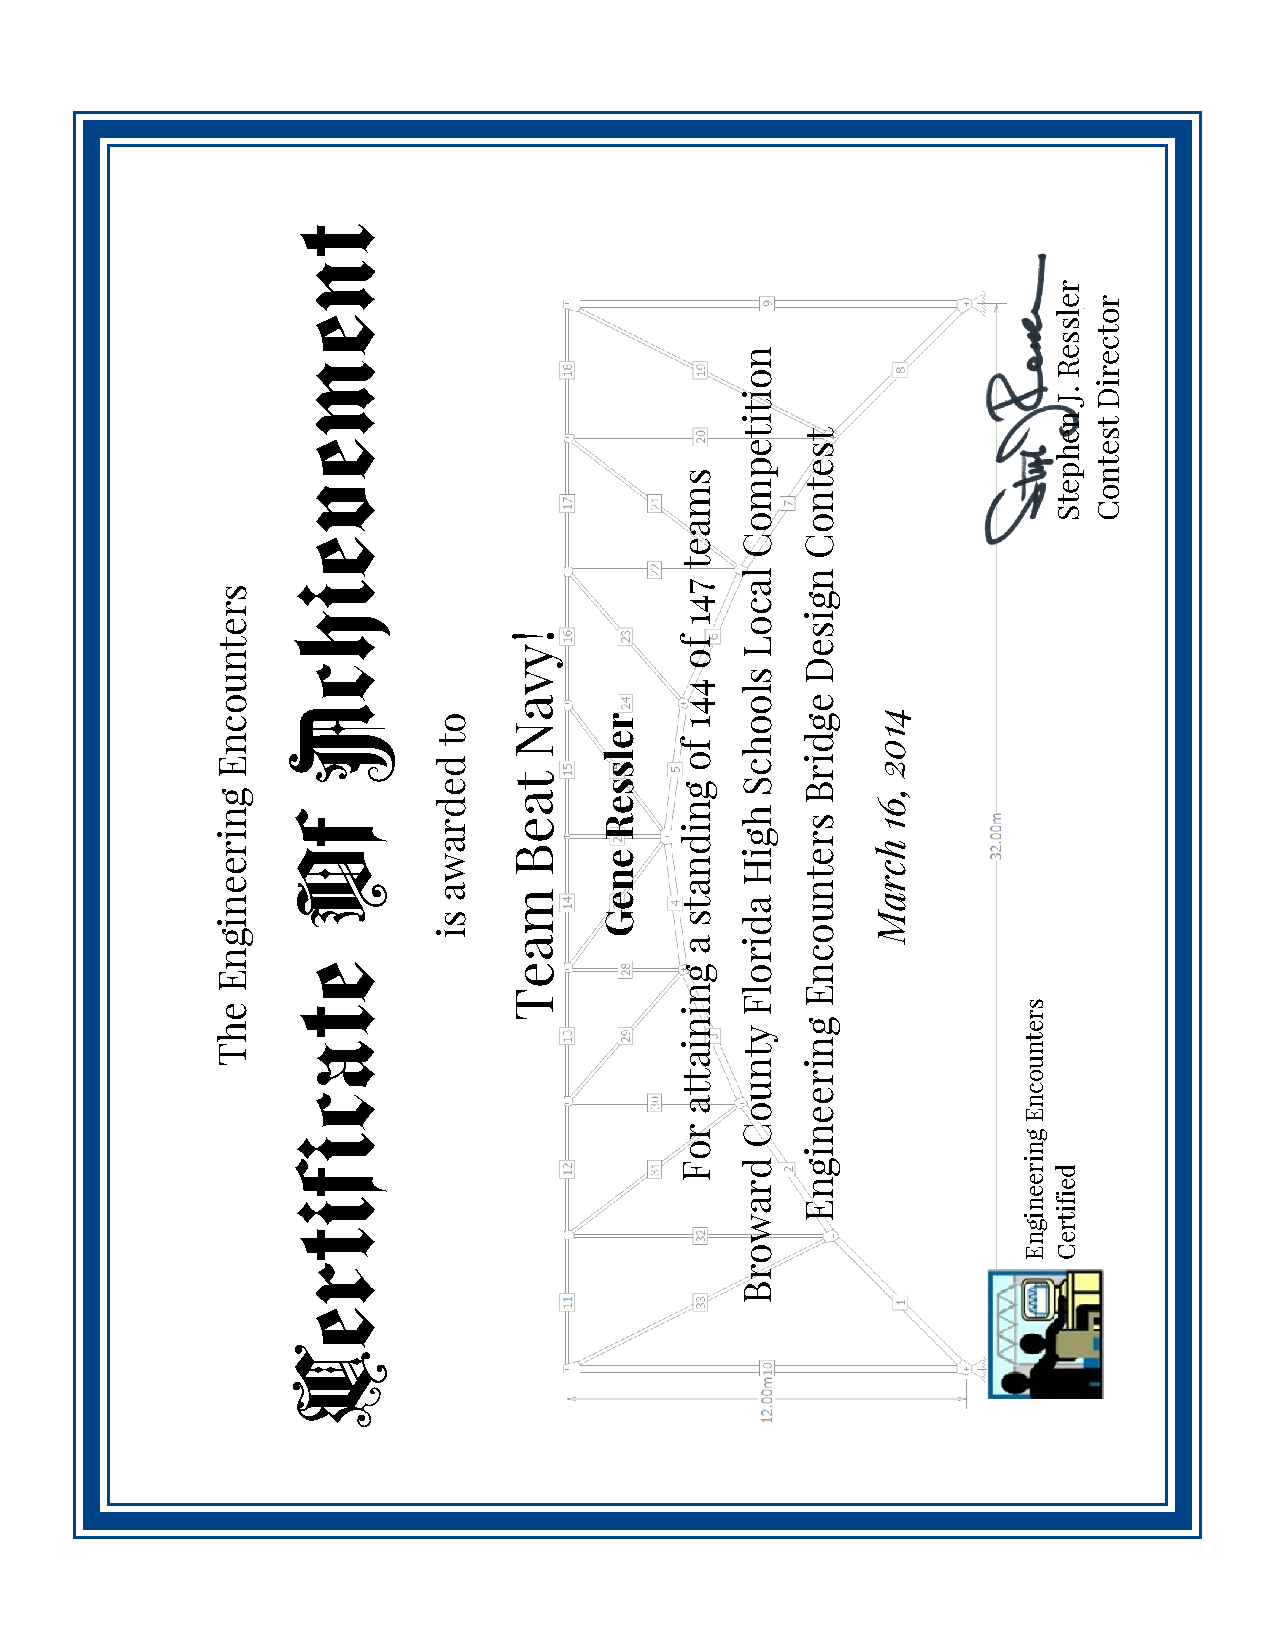
\includepdf[angle=90]{localcontestcertificate.pdf}
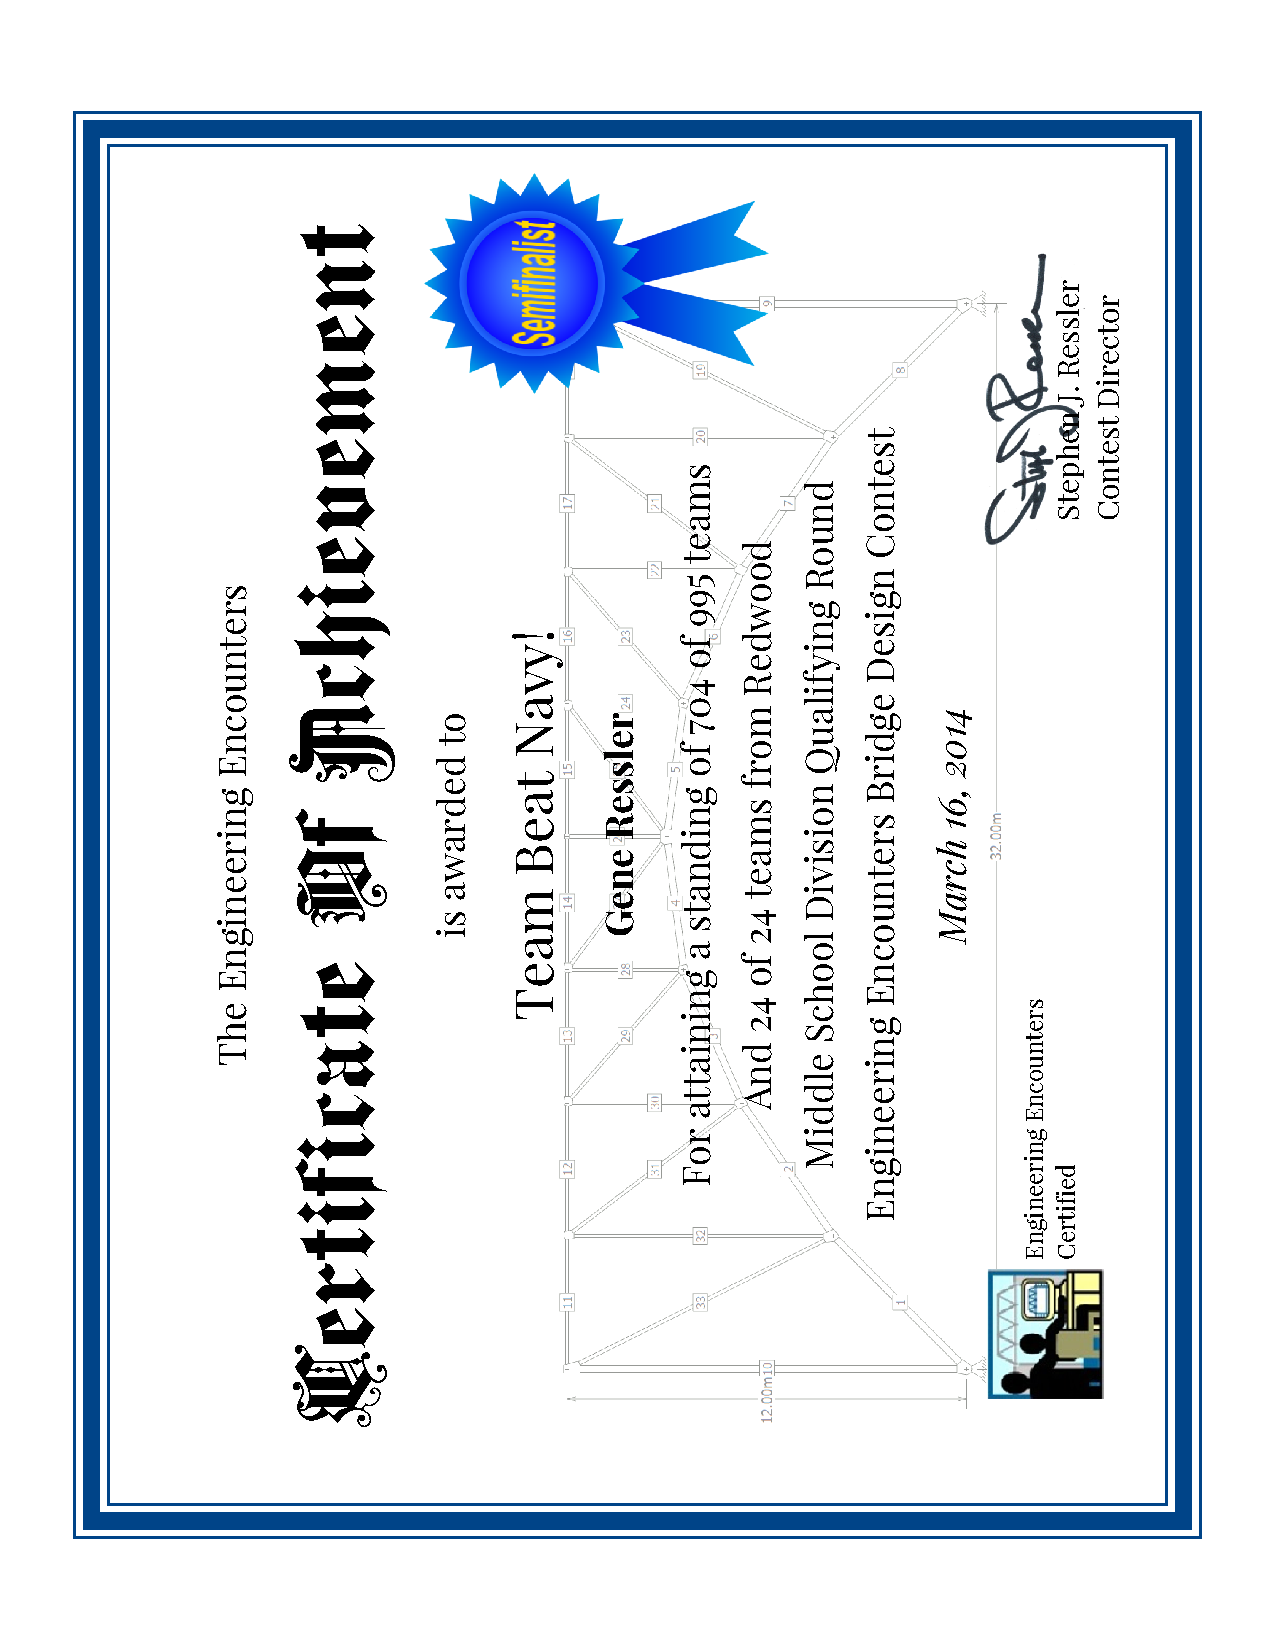
\includepdf[angle=90]{qualifierscertificate.pdf}
\end{document}  